%% Creator: Inkscape inkscape 0.48.0, www.inkscape.org
%% PDF/EPS/PS + LaTeX output extension by Johan Engelen, 2010
%% Accompanies image file 'pic1HARM_L3+L1RAD.ps' (pdf, eps, ps)
%%
%% To include the image in your LaTeX document, write
%%   \input{<filename>.pdf_tex}
%%  instead of
%%   \includegraphics{<filename>.pdf}
%% To scale the image, write
%%   \def\svgwidth{<desired width>}
%%   \input{<filename>.pdf_tex}
%%  instead of
%%   \includegraphics[width=<desired width>]{<filename>.pdf}
%%
%% Images with a different path to the parent latex file can
%% be accessed with the `import' package (which may need to be
%% installed) using
%%   \usepackage{import}
%% in the preamble, and then including the image with
%%   \import{<path to file>}{<filename>.pdf_tex}
%% Alternatively, one can specify
%%   \graphicspath{{<path to file>/}}
%% 
%% For more information, please see info/svg-inkscape on CTAN:
%%   http://tug.ctan.org/tex-archive/info/svg-inkscape

\begingroup
  \makeatletter
  \providecommand\color[2][]{%
    \errmessage{(Inkscape) Color is used for the text in Inkscape, but the package 'color.sty' is not loaded}
    \renewcommand\color[2][]{}%
  }
  \providecommand\transparent[1]{%
    \errmessage{(Inkscape) Transparency is used (non-zero) for the text in Inkscape, but the package 'transparent.sty' is not loaded}
    \renewcommand\transparent[1]{}%
  }
  \providecommand\rotatebox[2]{#2}
  \ifx\svgwidth\undefined
    \setlength{\unitlength}{250.77832031pt}
  \else
    \setlength{\unitlength}{\svgwidth}
  \fi
  \global\let\svgwidth\undefined
  \makeatother
  \begin{picture}(1,0.77024264)%
    \put(0,0){\includegraphics[width=\unitlength]{pics/pic1HARM_L3+L1RAD.ps}}%
    \put(0.52,0.008){\color[rgb]{0,0,0}\makebox(0,0)[lb]{\smash{$r$\,(см)}}}%
    \put(0.142,0.10032827){\color[rgb]{0,0,0}\makebox(0,0)[lb]{\smash{$-10$}}}%
    \put(0.35,0.10032827){\color[rgb]{0,0,0}\makebox(0,0)[lb]{\smash{$-5$}}}%
    \put(0.57350524,0.10032827){\color[rgb]{0,0,0}\makebox(0,0)[lb]{\smash{$0$}}}%
    \put(0.77172397,0.10032827){\color[rgb]{0,0,0}\makebox(0,0)[lb]{\smash{$5$}}}%
    \put(0.9576615,0.10032827){\color[rgb]{0,0,0}\makebox(0,0)[lb]{\smash{$10$}}}%
    \put(0.02666075,0.38){\color[rgb]{0,0,0}\rotatebox{90}{\makebox(0,0)[lb]{\smash{$\Delta{}B$\,(мГс)}}}}%
    \put(0.09684225,0.16022851){\color[rgb]{0,0,0}\makebox(0,0)[lb]{\smash{$-15$}}}%
    \put(0.09610548,0.33677886){\color[rgb]{0,0,0}\makebox(0,0)[lb]{\smash{$-10$}}}%
    \put(0.11918519,0.51379582){\color[rgb]{0,0,0}\makebox(0,0)[lb]{\smash{$-5$}}}%
    \put(0.15,0.69034607){\color[rgb]{0,0,0}\makebox(0,0)[lb]{\smash{$0$}}}%
    \put(0.79865731,0.54693785){\color[rgb]{0,0,0}\makebox(0,0)[lb]{\smash{$(1)$}}}%
    \put(0.73485594,0.61711936){\color[rgb]{0,0,0}\makebox(0,0)[lb]{\smash{$(2)$}}}%
  \end{picture}%
\endgroup
